\documentclass[10pt]{article}
\usepackage[paperwidth=16cm,paperheight=5.5cm,margin=0.1cm]{geometry}
\usepackage{fontspec}
\setmainfont{lmroman10-regular.otf}[BoldFont=lmroman10-bold.otf]
\usepackage{amsmath,amssymb,tikz}
\usetikzlibrary{arrows.meta,decorations.pathreplacing}
\pagestyle{empty}\setlength{\parindent}{0pt}
\begin{document}
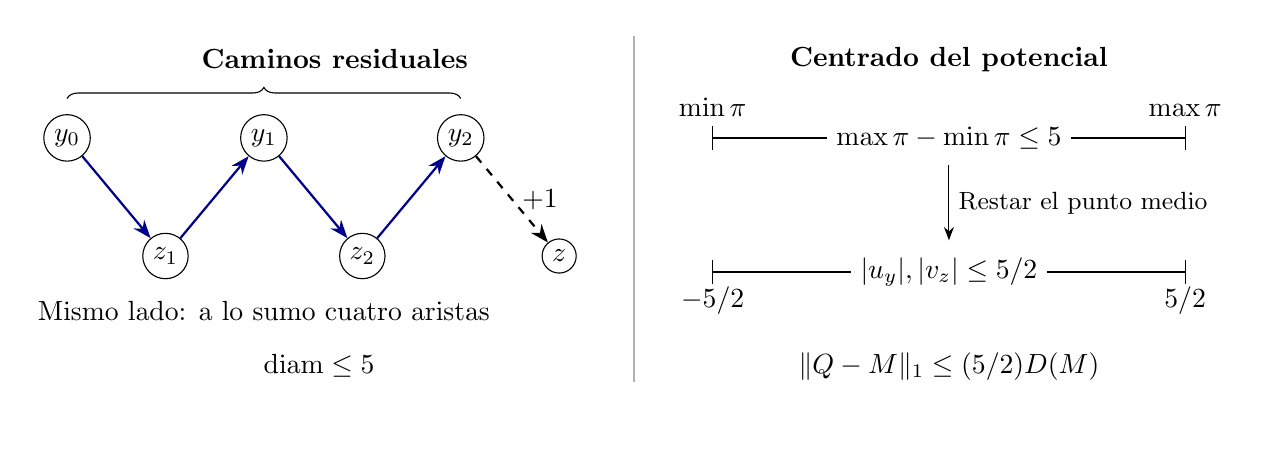
\begin{tikzpicture}[x=1cm,y=1cm,>=Stealth,vertex/.style={circle,draw,fill=white,inner sep=2pt}]
\useasboundingbox (-0.5,-1.4) rectangle (15.1,3.6);
\node[font=\bfseries] at (3.4,3.2) {Caminos residuales};
\node[vertex] (a) at (0,2.2) {$y_0$};
\node[vertex] (b) at (1.25,0.7) {$z_1$};
\node[vertex] (c) at (2.5,2.2) {$y_1$};
\node[vertex] (d) at (3.75,0.7) {$z_2$};
\node[vertex] (e) at (5,2.2) {$y_2$};
\node[vertex] (f) at (6.25,0.7) {$z$};
\draw[->,thick,blue!55!black] (a)--(b);
\draw[->,thick,blue!55!black] (b)--(c);
\draw[->,thick,blue!55!black] (c)--(d);
\draw[->,thick,blue!55!black] (d)--(e);
\draw[->,thick,dashed] (e)--(f) node[midway,right] {$+1$};
\draw[decorate,decoration={brace,amplitude=4pt}] (0,2.7)--(5,2.7);
\node[align=center] at (2.5,0) {Mismo lado: a lo sumo cuatro aristas};
\node at (3.2,-0.7) {$\operatorname{diam}\le 5$};
\draw[gray!60] (7.2,-0.9)--(7.2,3.5);
\node[font=\bfseries] at (11.2,3.2) {Centrado del potencial};
\draw[thick] (8.2,2.2)--(14.2,2.2);
\draw (8.2,2.05)--(8.2,2.35) node[above] {$\min\pi$};
\draw (14.2,2.05)--(14.2,2.35) node[above] {$\max\pi$};
\node[fill=white] at (11.2,2.2) {$\max\pi-\min\pi\le 5$};
\draw[->] (11.2,1.85)--(11.2,0.9) node[midway,right,font=\small] {Restar el punto medio};
\draw[thick] (8.2,0.5)--(14.2,0.5);
\draw (8.2,0.35)--(8.2,0.65) node[below=6pt] {$-5/2$};
\draw (14.2,0.35)--(14.2,0.65) node[below=6pt] {$5/2$};
\node[fill=white] at (11.2,0.5) {$|u_y|,|v_z|\le 5/2$};
\node at (11.2,-0.7) {$\|Q-M\|_1\le (5/2)D(M)$};
\end{tikzpicture}
\end{document}
